\documentclass[allowframebreaks,10pt]{beamer}
\usetheme{Madrid}
\usefonttheme{serif}
\usepackage{listings}
\usepackage[slantfont, boldfont, CJKtextspaces, CJKmathspaces]{xeCJK}
\usepackage{fontspec,xunicode,xltxtra}
\usepackage{indentfirst}
\usepackage{color}
\usepackage{alltt}
\usepackage{marvosym}
\usepackage{amsmath}

\setCJKmainfont[BoldFont={黑体}, ItalicFont={楷体_GB2312}]{宋体}
%\setmainfont{Liberation Serif} 
%\setsansfont{Liberation Sans} 
\setmonofont{YaHei Consolas Hybrid}

\punctstyle{kaiming} % 开明式标点格式  

\title[FFT对某种特定DP的优化]{FFT对某种特定DP的优化}
\author[csimstu,zcwwzdjn]{\small\itshape{李凌霄,王迪}}
\institute[CDQZ]{
	{\small\itshape 成都七中} \\[0.5ex]
		\texttt{csimstu@gmail.com, zcwwzdjn@hotmail.com}
}

\begin{document}

\begin{frame}[plain]
\titlepage
\end{frame}

\begin{frame}[plain]
\begin{center}
\textbf{第一部分:多项式与FFT}
\end{center}
\end{frame}

\begin{frame}{多项式}
一个多项式(polynomial)$A(x)$是一个函数\footnote{假定多项式长度相等,均为$n$,且$n=2^t$}:
\[
A(x) = \sum_{j=0}^{n-1}a_j x^{j}
\]
\pause
多项式的加法、乘法:
\[
C(x) = A(x) + B(x) \to c_j = a_j + b_j 
\]
\[
C(x) = A(x)B(x) \to c_j = \sum_{k=0}^{j} a_k b_{j-k}
\]
\end{frame}

\begin{frame}{多项式的表示}
\begin{itemize}
\pause
\item 系数表示法(Coffecient representation)
\[
A(x) = \sum_{j=0}^{n-1}a_j x^{j}
\]
\pause
\item 点值表示法(Point-value representation)
	\\ 用$n$个二元组来表示一个多项式:
	\[
	\{ (x_0, y_0), (x_1, y_1), (x_2, y_2), \ldots, (x_{n-1}, y_{n-1})\}
	\]
	满足对所有的$k$,$x_k$互不相等且$y_k = A(x_k)$。
	\pause
	可以证明,点值表示法可以对应一个唯一的系数表示法。
\end{itemize}

\end{frame}

\begin{frame}{对比两种表示方法}
\begin{itemize}
\pause
\item 求值
	\[ O(n) < O(?)\]
\pause
\item 多项式加法
	\[O(n) = O(n)\]
\pause
\item 多项式乘法
	\[ O(n^2) > O(n) \]
\pause
\item 多项式自乘$k$次
	\[ O(kn^2) \gg O(n \log k) \]
\end{itemize}
\pause
\textbf{点值表示法是多项式运算的核心。}
\end{frame}

\begin{frame}{两种表示方法相互转化}
\begin{itemize}
\pause
\item 系数to点值 
\pause
	\\[1ex] 任取$n$个不同的数作为${x}$,$O(n^2)$
\pause
\item 点值to系数
\pause
	\\[1ex] 解方程 $O(n^3)$
\pause
	\\ Lagrange’s formula $O(n^2)$
\end{itemize}
\pause
毫无疑问,以上方法都太慢了!
\end{frame}

\begin{frame}{引入FFT}
快速傅里叶变化(Fast Fourier Transforms)是一种能在
$O(n \log n)$时间内实现两种转化的技术。
\pause
\\ 我们注意到,$\{x\}$的选值是可以人为操控的,还有很大的利用余地。
\pause
一种比较好的方法是选用$\omega ^n = 1$的$n$个复数根。
\end{frame}

\begin{frame}{复数基础}
\pause
复单位:$i$,定义$i^2=-1$。 \\
\pause
复平面: \\
		\begin{center}
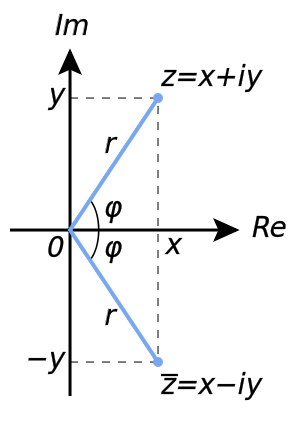
\includegraphics[width=0.3\textwidth]{300px-Complex_conjugate_picture.svg.png} \\
					   \end{center}
\pause
复数的四则运算:直接推。 \\
\pause
如何实现?\pause \\
重载运算(封装)。
\end{frame}

\begin{frame}{复数基础}
欧拉公式:
\[ e ^{i \theta } = \cos \theta + i \sin \theta \]
单位根:
\[ \omega_n = e ^ {2 \pi i / n}\]
\pause
$\omega ^ n = 1$的$n$个复数根可以表示为
\[ \omega_n^0, \omega_n^1, \ldots, \omega_n^{n-1}\]

\pause
优秀性质:
\begin{itemize}
\pause
\item 周期性:$\omega_n^{j+kn} = \omega_n^j$
\pause
\item 消除性:$\omega_{dn}^{dk} = \omega_n^k$
\pause
\item 和为零:$\sum_{j=0}^{n-1} (\omega_n^k)^j = 0$
\end{itemize}
\end{frame}

\begin{frame}{It's show time}
约定系数to点值称为DFT,点值to系数称为IDFT。
\pause
对每个$k$,我们实际上是要计算$y_k = A(\omega_n^k) = \sum_{j=0}^{n-1}a_j \omega_n^{kj}$。
\pause
\\ 将多项式$A$按奇偶分解:
\pause
\[ A^{[0]}(x) = a_0 + a_2x + a_4x^2 + \ldots + 
a_{n-2}x^{n/2-1}\]
\pause
\[ A^{[1]}(x) = a_1 + a_3x + a_5x^2 + \ldots + 
a_{n-1}x^{n/2-1}\]
\pause
于是:
\[ A(x) = A^{[0]}(x^2) + x A^{[1]}(x^2)\]。
\pause
将$x=\omega_n^k$代入:
\[ A(\omega_n^k) = A^{[0]}(\omega_n^{2k}) + \omega_n^k A^{[1]}(\omega_n^{2k})\]。
\pause
由消除性,可得:
\[ A(\omega_n^k) = A^{[0]}(\omega_{n/2}^{k}) + \omega_n^k A^{[1]}(\omega_{n/2}^{k})\]。
\pause
注意到多项式$A^{[0]}$与$A^{[1]}$都只有$n/2$项,若$k \ge n/2$有$\omega_{n/2}^k = \omega_{n/2}^{k-n/2}$。
\pause
问题被完美的转化为了子问题!系数到点值的转化就能在$O(n \log n)$时间内进行了。
\end{frame}
\begin{frame}{逆转化}
\pause
一个结论(证明略去):
\[ a_j = \frac{1}{n} \sum_{k=0}^{n-1} y_k \omega_n^{-kj}\]
\pause
跟刚才的形式如出一辙。我们只需要将$\omega_n$替换为$\omega_n^{-1}$,
最后全部除以$n$就解决了。
\end{frame}

\begin{frame}{code}
基本的FFT只需10行:\\[1ex]
{\footnotesize
% Style definition file generated by highlight 3.9, http://www.andre-simon.de/ 

% Highlighting theme: Gedit Editor 

\newcommand{\hlstd}[1]{\textcolor[rgb]{0.23,0.22,0.21}{#1}}
\newcommand{\hlnum}[1]{\textcolor[rgb]{1,0,1}{#1}}
\newcommand{\hlesc}[1]{\textcolor[rgb]{1,0,1}{#1}}
\newcommand{\hlstr}[1]{\textcolor[rgb]{1,0,1}{#1}}
\newcommand{\hlpps}[1]{\textcolor[rgb]{1,0,1}{#1}}
\newcommand{\hlslc}[1]{\textcolor[rgb]{0,0.24,1}{#1}}
\newcommand{\hlcom}[1]{\textcolor[rgb]{0,0.24,1}{#1}}
\newcommand{\hlppc}[1]{\textcolor[rgb]{0.63,0.13,0.94}{#1}}
\newcommand{\hlopt}[1]{\textcolor[rgb]{0.23,0.22,0.21}{#1}}
\newcommand{\hllin}[1]{\textcolor[rgb]{0.24,0.23,0.22}{#1}}
\newcommand{\hlkwa}[1]{\textcolor[rgb]{0.65,0.16,0.21}{#1}}
\newcommand{\hlkwb}[1]{\textcolor[rgb]{0.18,0.55,0.34}{#1}}
\newcommand{\hlkwc}[1]{\textcolor[rgb]{0.34,0.18,0.55}{#1}}
\newcommand{\hlkwd}[1]{\textcolor[rgb]{0.23,0.22,0.21}{\bf{#1}}}
\definecolor{bgcolor}{rgb}{1,1,1}



\pagecolor{bgcolor}
\newsavebox{\hlboxopenbrace}
\newsavebox{\hlboxclosebrace}
\newsavebox{\hlboxlessthan}
\newsavebox{\hlboxgreaterthan}
\newsavebox{\hlboxdollar}
\newsavebox{\hlboxunderscore}
\newsavebox{\hlboxand}
\newsavebox{\hlboxhash}
\newsavebox{\hlboxat}
\newsavebox{\hlboxbackslash}
\newsavebox{\hlboxpercent}
\newsavebox{\hlboxhat}
\setbox\hlboxopenbrace=\hbox{\verb.{.}
\setbox\hlboxclosebrace=\hbox{\verb.}.}
\setbox\hlboxlessthan=\hbox{\verb.<.}
\setbox\hlboxgreaterthan=\hbox{\verb.>.}
\setbox\hlboxdollar=\hbox{\verb.$.}
\setbox\hlboxunderscore=\hbox{\verb._.}
\setbox\hlboxand=\hbox{\verb.&.}
\setbox\hlboxhash=\hbox{\verb.#.}
\setbox\hlboxat=\hbox{\verb.@.}
\setbox\hlboxbackslash=\hbox{\verb.\.}
\setbox\hlboxpercent=\hbox{\verb.\%.}
\setbox\hlboxhat=\hbox{\verb.^.}
\def\urltilda{\kern -.15em\lower .7ex\hbox{\~{}}\kern .04em}
\noindent
\ttfamily
\hlstd{}\hlkwb{void\ }\hlstd{}\hlkwd{fft}\hlstd{}\hlopt{(}\hlstd{}\hlkwb{int\ }\hlstd{delta}\hlopt{,\ }\hlstd{}\hlkwb{int\ }\hlstd{step}\hlopt{,\ }\hlstd{}\hlkwb{int\ }\hlstd{size}\hlopt{,\ }\hlstd{}\hlkwb{int\ }\hlstd{flag}\hlopt{)\ \usebox{\hlboxopenbrace}}\hspace*{\fill}\\
\hlstd{}\hlstd{\ \ \ \ }\hlstd{}\hlkwa{if\ }\hlstd{}\hlopt{(\ }\hlstd{size\ }\hlopt{==\ }\hlstd{}\hlnum{1\ }\hlstd{}\hlopt{)\ \usebox{\hlboxopenbrace}\ }\hlstd{res}\hlopt{{[}}\hlstd{delta}\hlopt{{]}\ =\ }\hlstd{coef}\hlopt{{[}}\hlstd{delta}\hlopt{{]};\ }\hlstd{}\hlkwa{return}\hlstd{}\hlopt{;\ \usebox{\hlboxclosebrace}}\hspace*{\fill}\\
\hlstd{}\hlstd{\ \ \ \ }\hlstd{}\hlkwd{fft}\hlstd{}\hlopt{(}\hlstd{delta}\hlopt{,\ }\hlstd{step\ }\hlopt{{*}\ }\hlstd{}\hlnum{2}\hlstd{}\hlopt{,\ }\hlstd{size\ }\hlopt{/\ }\hlstd{}\hlnum{2}\hlstd{}\hlopt{,\ }\hlstd{flag}\hlopt{);}\hspace*{\fill}\\
\hlstd{}\hlstd{\ \ \ \ }\hlstd{}\hlkwd{fft}\hlstd{}\hlopt{(}\hlstd{delta\ }\hlopt{+\ }\hlstd{step}\hlopt{,\ }\hlstd{step\ }\hlopt{{*}\ }\hlstd{}\hlnum{2}\hlstd{}\hlopt{,\ }\hlstd{size\ }\hlopt{/\ }\hlstd{}\hlnum{2}\hlstd{}\hlopt{,\ }\hlstd{flag}\hlopt{);}\hspace*{\fill}\\
\hlstd{}\hlstd{\ \ \ \ }\hlstd{Complex\ }\hlkwd{acc}\hlstd{}\hlopt{(}\hlstd{}\hlnum{1}\hlstd{}\hlopt{,\ }\hlstd{}\hlnum{0}\hlstd{}\hlopt{),\ }\hlstd{}\hlkwd{pri}\hlstd{}\hlopt{(}\hlstd{}\hlkwd{cos}\hlstd{}\hlopt{(}\hlstd{flag\ }\hlopt{{*}\ }\hlstd{}\hlnum{2\ }\hlstd{}\hlopt{{*}\ }\hlstd{PI\ }\hlopt{/\ }\hlstd{size}\hlopt{),\ }\hlstd{}\hlkwd{sin}\hlstd{}\hlopt{(}\hlstd{flag\ }\hlopt{{*}\ }\hlstd{}\hlnum{2\ }\hlstd{}\hlopt{{*}\ }\hlstd{PI\ }\hlopt{/\ }\hlstd{size}\hlopt{));}\hspace*{\fill}\\
\hlstd{}\hlstd{\ \ \ \ }\hlstd{}\hlkwa{for\ }\hlstd{}\hlopt{(\ }\hlstd{}\hlkwb{int\ }\hlstd{i\ }\hlopt{=\ }\hlstd{}\hlnum{0}\hlstd{}\hlopt{;\ }\hlstd{i\ }\hlopt{\usebox{\hlboxlessthan}\ }\hlstd{size\ }\hlopt{/\ }\hlstd{}\hlnum{2}\hlstd{}\hlopt{;\ }\hlstd{i\ }\hlopt{++,\ }\hlstd{acc\ }\hlopt{=\ }\hlstd{acc\ }\hlopt{{*}\ }\hlstd{pri\ }\hlopt{)\ }\hspace*{\fill}\\
\hlstd{}\hlstd{\ \ \ \ \ \ \ \ }\hlstd{tmp}\hlopt{{[}}\hlstd{delta\ }\hlopt{+\ }\hlstd{i\ }\hlopt{{*}\ }\hlstd{step}\hlopt{{]}\ =\ }\hlstd{res}\hlopt{{[}}\hlstd{delta\ }\hlopt{+\ }\hlstd{i\ }\hlopt{{*}\ }\hlstd{step\ }\hlopt{{*}\ }\hlstd{}\hlnum{2}\hlstd{}\hlopt{{]}\ +\ }\hlstd{acc\ }\hlopt{{*}\ }\hlstd{res}\hlopt{{[}}\hlstd{delta\ }\hlopt{+\ }\hlstd{step\ }\hlopt{+\ }\hlstd{i\ }\hlopt{{*}\ }\hlstd{step\ }\hlopt{{*}\ }\hlstd{}\hlnum{2}\hlstd{}\hlopt{{]};}\hspace*{\fill}\\
\hlstd{}\hlstd{\ \ \ \ }\hlstd{}\hlkwa{for\ }\hlstd{}\hlopt{(\ }\hlstd{}\hlkwb{int\ }\hlstd{i\ }\hlopt{=\ }\hlstd{size\ }\hlopt{/\ }\hlstd{}\hlnum{2}\hlstd{}\hlopt{;\ }\hlstd{i\ }\hlopt{\usebox{\hlboxlessthan}\ }\hlstd{size}\hlopt{;\ }\hlstd{i\ }\hlopt{++,\ }\hlstd{acc\ }\hlopt{=\ }\hlstd{acc\ }\hlopt{{*}\ }\hlstd{pri\ }\hlopt{)\ }\hspace*{\fill}\\
\hlstd{}\hlstd{\ \ \ \ \ \ \ \ }\hlstd{tmp}\hlopt{{[}}\hlstd{delta\ }\hlopt{+\ }\hlstd{i\ }\hlopt{{*}\ }\hlstd{step}\hlopt{{]}\ =\ }\hlstd{res}\hlopt{{[}}\hlstd{delta\ }\hlopt{+\ (}\hlstd{i\ }\hlopt{{-}\ }\hlstd{size\ }\hlopt{/\ }\hlstd{}\hlnum{2}\hlstd{}\hlopt{)\ {*}\ }\hlstd{step\ }\hlopt{{*}\ }\hlstd{}\hlnum{2}\hlstd{}\hlopt{{]}\ +\ }\hlstd{acc\ }\hlopt{{*}\ }\hlstd{res}\hlopt{{[}}\hlstd{delta\ }\hlopt{+\ }\hlstd{step\ }\hlopt{+\ (}\hlstd{i\ }\hlopt{{-}\ }\hlstd{size\ }\hlopt{/\ }\hlstd{}\hlnum{2}\hlstd{}\hlopt{)\ {*}\ }\hlstd{step\ }\hlopt{{*}\ }\hlstd{}\hlnum{2}\hlstd{}\hlopt{{]};}\hspace*{\fill}\\
\hlstd{}\hlstd{\ \ \ \ }\hlstd{}\hlkwa{for\ }\hlstd{}\hlopt{(\ }\hlstd{}\hlkwb{int\ }\hlstd{i\ }\hlopt{=\ }\hlstd{}\hlnum{0}\hlstd{}\hlopt{;\ }\hlstd{i\ }\hlopt{\usebox{\hlboxlessthan}\ }\hlstd{size}\hlopt{;\ }\hlstd{i\ }\hlopt{++\ )\ }\hlstd{res}\hlopt{{[}}\hlstd{delta\ }\hlopt{+\ }\hlstd{i\ }\hlopt{{*}\ }\hlstd{step}\hlopt{{]}\ =\ }\hlstd{tmp}\hlopt{{[}}\hlstd{delta\ }\hlopt{+\ }\hlstd{i\ }\hlopt{{*}\ }\hlstd{step}\hlopt{{]};}\hspace*{\fill}\\
\hlstd{}\hlopt{\usebox{\hlboxclosebrace}}\hlstd{}\hspace*{\fill}\\
\mbox{}
\normalfont
\normalsize

}
\end{frame}

\begin{frame}[plain]
\begin{center}
\textbf{第二部分:例题*6}
\end{center}
\end{frame}

\begin{frame}{eg0.高精度乘法}
\begin{example}
给两个50000位左右的正整数,算它们的乘积。
\end{example}
\pause
\begin{solution}
把正整数表示成多项式$f(x)$,使得代入$x=10$得到原来的数,于是原来整数的每一位都是多项式中它对应的那一项的系数,然后利用FFT做多项式乘法即可。
\\ 大家可以到HDU1402验证自己的正确性。
\end{solution}
\pause
ext:可以考虑压位来加速。\\
\pause
extext:FFT后得到的数组中实数的范围会不会超过int? \\
\pause
extextext:有没有办法可以在一定程度上消除精度误差? 
\end{frame}


\begin{frame}{eg1.SPOJ TSUM}
\begin{example}
给定40000个绝对值不超过20000且互不相同的整数,考虑下标三元组$(a,b,c)$,其中$a,b,c$互不相同,其权值为对应3个数的和,
	对每个可能的权值统计无序三元组(即$(a,b,c)=(b,a,c)=\ldots$)。
\end{example}
Hint: 若$a,b,c$有序且不必互不相同,有没有办法?
\end{frame}

\begin{frame}{eg2. CTSC2010 性能优化}
\begin{example}
定义一个算法,$f[i+1][(j+k)\%n]=\sum f[i][j] \times g[k] \% (n+1)$,保证$n+1$为质数,且$n$最大的质因子不超过7。
给出$n,c,f[0]$数组和$g$数组,计算$f[c]$数组,其中$n \le 5 \times 10^5, c \le 10^9$。
\end{example}
Hint: 先不考虑答案要模$n+1$,如何计算$f[i+1][(j+k)\%n]=\sum f[i][j] \times g[k]$?
\end{frame}

\begin{frame}{eg2. CTSC2010 性能优化}
ext:注意到这题的$n$不是2的幂,但满足最大的质因子不超过7,怎么破? \\
\pause
extext:若前两个问题都解决了,可以考虑做今年集训队答辩中伍一鸣的Binomial。
\end{frame}


\begin{frame}{eg3. TopCoder SRM 518 DIV1 Nim}
\begin{example}
两人玩Nim游戏,桌上有不超过$10^9$堆石子,每堆石子的个数是质数且不超过$5 \times 10^4$。问有多少种情况使得后手必胜?
\end{example}
\pause
Hint:能不能写出DP的方程? \newline
\pause
我们注意到这和多项式乘法很相似,只不过下标变化从$j+k$变成了$j\oplus k$,于是我们考虑转化。 \\
\pause
我们用$\star$符号来表示两个数组的某种运算,$\star$的两个参数是数组,返回的也是数组。上式可以描述为$f[i+1]=f[i]\star g$。\\
定义:\\
用大写字母表示数组,用小写字母表示数字,$[\ldots]$表示数组,比如$A=[a,b]$。\\
数组的含义:下标从0开始,$A[x]$表示xor起来为$x$的方案数。\\
$(A\times B)[i]=A[i]\times B[i]$ \\
$(A+B)[i]=A[i]+B[i]$ \\
\end{frame}
\begin{frame}{eg3. TopCoder SRM 518 DIV1 Nim}
考虑多项式乘法,$\star$的含义就是对两个数组做多项式的乘法,在过程中我们有 \\
$DFT(A \star B)=DFT(A)\times DFT(B)$,
$IDFT(DFT(A))=A$。\\
\pause
考虑现在的问题,我们能否找到一种转换方式使得$tf(A\star B)=tf(A) \times tf(B), utf(tf(A))=A$?\\
猜测tf可能与utf类似,我们重点考虑tf。\\
\pause
显然$tf([a])=[a]$。$tf([a,b])$是什么呢?\\
\end{frame}

\begin{frame}{eg3. TopCoder SRM 518 DIV1 Nim}
Hint: 考虑$[a,b] \star [c,d]$。\\
Hint: 猜测$tf([a,b])$的两项都是关于$a$和$b$的线性函数。\\
\pause
其实$tf([a,b])=[a+b,a-b]$。\\
\pause
进一步猜测:$tf([A,B])=[tf(A)+tf(B),tf(A)-tf(B)]$, \\ 
证明?\\
\pause
ext:这题是异或、逻辑与、逻辑或等运算是不是也可以做呢?
\end{frame}

\begin{frame}{eg4. TopCoder TCO12 Round2A EvenPaths}
\begin{example}
给一个点数不超过50的DAG,有一些点是空地有一些是障碍,还有一些是未探明的区域。设未探明的区域有$k$个,$k$不会超过32,那么DAG就有$2^k$种可能。我们考虑这$2^k$种情况中,有多少使得从0到1的路径数是偶数?
\end{example}
\pause
Hint:对一个确定的图,如何计算0到1的路径数的奇偶性? \\
\pause
Hint:枚举$2^{32}$次方是不可能的,能否通过折半,枚举$2^{16}$再将两边合并?
\pause
对图进行拓扑排序,把32个点分为两个集合$A$和$B$,A包含前16个点,B包含后16个点。\\
考虑$S$为$B$集合加上1号点。\\
这样有很好的一个性质,就是从0走到1,必定经过$S$集合中至少1个点。\\
于是我们可以通过考虑从0到1碰到$S$中第一个点来对所有的路径进行计数。\\
\pause
注意到奇偶是一个01变量,能不能通过状态压缩来进行动态规划?\\
考虑枚举$B$集合后,$S$集合中的每点走到1号点路径数的奇偶性用一个长度为17的二进制数来表示。\\
\pause
用f[mask]来表示使mask这种情况发生的$B$集合状态数。\\
\end{frame}

\begin{frame}{Summary}
以上几道题向我们展示了FFT可以优化某种特定的DP,它们都具有以下共性:
\pause
\begin{enumerate}
\item 状态本质为一维。 
\pause
\item 具有$C[i \star j] = A[i] \times B[j]$的形式。
$\star$可以为加法、带模加法、按位异或、按位与,等等。
\pause
\item 优化的过程都是转化成类点值表示法\textbf{解耦合},然后每对点值\textbf{独立运算},再转化回去。
\pause
\item 转化与逆转化都借用了分而治之的思想。
\end{enumerate}
\end{frame}

\begin{frame}{More Exercises}
CDOJ1714 Graph Game,CDOJ是UESTC的OJ。
\end{frame}

\begin{frame}{CDOJ1714 Graph Game}
\begin{example}
A与B在一个无向图上做一个游戏。A与B轮流操作,A先手。
每次删掉一条边,满足该边连接的两个点度和为偶数。
谁不能找到这样合法的边谁就输。
\\ 现在,他们得到了一个包含$n$个点$m$条边的无向图。
A想知道,有多少子图使得他能获胜?(两人都以最优策略删边)
\\ $2 \le n \le 40, 1 \le m \le 400$
\end{example}

\pause
先手必胜的条件?
\pause
如何利用FFT优化?

\end{frame}

\end{document}
